% Meeting → Slides POC — extended technical documentation
% Engine: pdfLaTeX (MiKTeX / TeX Live). Run twice for TOC and references.
\documentclass[11pt,a4paper]{article}

\usepackage[T1]{fontenc}
\usepackage[utf8]{inputenc}
\usepackage[english]{babel}
\usepackage[margin=24mm,bindingoffset=0mm]{geometry}

% Typography (Charter + matching math — readable on screen and print)
\usepackage[bitstream-charter]{mathdesign}
\usepackage{microtype}
\usepackage{setspace}
\setstretch{1.06}

% Structure & layout
\usepackage{titlesec}
\usepackage{fancyhdr}
\usepackage{lastpage}
\usepackage{parskip}
\usepackage{enumitem}
\setlist{itemsep=0.25em,parsep=0pt,topsep=0.4em}

% Tables & code
\usepackage{booktabs}
\usepackage{tabularx}
\usepackage{array}
\usepackage{longtable}
\usepackage{xcolor}
% Colours (aligned with product UI: slate + teal) — before caption/listings use them
\definecolor{BrandTeal}{RGB}{34,160,150}
\definecolor{BrandSlate}{RGB}{30,41,59}
\definecolor{CodeBg}{RGB}{248,250,252}
\definecolor{LinkBlue}{RGB}{30,64,175}
\usepackage{listings}
\usepackage{caption}
\captionsetup{font=small,labelfont={bf,color=BrandTeal}}

% Coloured boxes
\usepackage[most]{tcolorbox}
\tcbset{
  colback=white,
  colframe=BrandSlate!55,
  arc=2pt,
  boxrule=0.6pt,
  left=8pt,right=8pt,top=6pt,bottom=6pt,
}

% Diagrams
\usepackage{tikz}
\usetikzlibrary{arrows.meta,positioning,fit,calc}

\lstdefinelanguage{json}{
  keywords={true,false,null},
  sensitive=false,
  comment=[l]{//},
  string=[b]",
  morestring=[b]',
}
\lstset{
  basicstyle=\ttfamily\footnotesize,
  breaklines=true,
  frame=single,
  framerule=0.4pt,
  rulecolor=\color{BrandSlate!25},
  backgroundcolor=\color{CodeBg},
  columns=fullflexible,
  keepspaces=true,
  showstringspaces=false,
  tabsize=2,
}

% Section titles
\titleformat{\section}
  {\normalfont\Large\bfseries\color{BrandSlate}}{\thesection}{0.6em}{}
  [\vspace{-0.2em}{\color{BrandTeal}\rule{\linewidth}{1.2pt}}]
\titleformat{\subsection}
  {\normalfont\large\bfseries\color{BrandSlate!90}}{\thesubsection}{0.5em}{}
\titleformat{\subsubsection}
  {\normalfont\normalsize\bfseries\color{BrandSlate!80}}{\thesubsubsection}{0.45em}{}

% Header / footer
\pagestyle{fancy}
\fancyhf{}
\fancyhead[L]{\small\textcolor{BrandSlate!70}{Meeting $\rightarrow$ Slides POC}}
\fancyhead[R]{\small\textcolor{BrandTeal}{\nouppercase{\leftmark}}}
\fancyfoot[C]{\small\textcolor{BrandSlate!50}{Page \thepage\ of \pageref*{LastPage}}}
\renewcommand{\headrulewidth}{0.4pt}
\renewcommand{\headrule}{\hbox to\headwidth{\color{BrandTeal!40}\leaders\hrule height \headrulewidth\hfill}}

% Hyperlinks (load last)
\usepackage[hidelinks]{hyperref}
\hypersetup{
  colorlinks=true,
  linkcolor=LinkBlue,
  urlcolor=BrandTeal,
  citecolor=BrandSlate,
  pdftitle={Meeting to Slides POC - Architecture and Robustness},
  pdfauthor={FulcrumLATAM / Main Street AI Advisors},
  pdfsubject={Technical documentation},
}

% Title page customisation
\newcommand{\DocumentTitle}{Meeting $\rightarrow$ Slides\\[0.35em]\Large Proof of Concept}
\newcommand{\DocumentSubtitle}{Architecture, behaviour, and design rationale for a robust briefing pipeline}

\begin{document}

% ---------- Title ----------
\begin{titlepage}
  \centering
  \vspace*{1.2cm}
  {\color{BrandTeal}\rule{0.35\textwidth}{4pt}}\par\vspace{1em}
  {\LARGE\bfseries\color{BrandSlate}\DocumentTitle\par}
  \vspace{0.8em}
  {\large\color{BrandSlate!80}\DocumentSubtitle\par}
  \vspace{2.2cm}
  \begin{tcolorbox}[width=0.88\textwidth,colback=BrandSlate!4,colframe=BrandTeal!50,arc=4pt,title={\textbf{Document abstract}}]
    This note describes an end-to-end system that ingests \textbf{meeting transcripts} or \textbf{media}, calls cloud speech and language models where configured, and produces \textbf{structured JSON} plus an editable \textbf{PowerPoint} deck. It explains \emph{how} each layer works and \emph{why} specific engineering choices improve \textbf{reliability}, \textbf{observability}, and \textbf{auditability} compared to a minimal demo.
  \end{tcolorbox}
  \vfill
  {\large FulcrumLATAM / Main Street AI Advisors\par}
  \vspace{0.5em}
  {\normalsize \today\par}
  \vspace{1.2cm}
\end{titlepage}

\tableofcontents
\clearpage

% =============================================================================
\section{Purpose and scope}
% =============================================================================

\subsection{What the product does}
The POC automates an internal workflow:
\begin{enumerate}[label=\textbf{\arabic*.}]
  \item \textbf{Ingest} a plain-text transcript, or \textbf{audio/video} (\texttt{mp4}, \texttt{webm}, \texttt{mp3}, \texttt{wav}, \texttt{m4a}, \ldots).
  \item \textbf{Normalize} text (strip mail/UI noise when present).
  \item \textbf{Summarize} into a fixed JSON schema (executive summary, objectives, actions, next steps, human-review notes) using \textbf{Google Gemini} (primary) or \textbf{OpenAI} (optional), or a \textbf{deterministic demo template} when no API keys are set.
  \item \textbf{Render} a \texttt{.pptx} via \texttt{python-pptx} and expose \textbf{download links} for transcript, JSON, and slides.
  \item \textbf{Stream progress} to the browser with \textbf{Server-Sent Events (SSE)} so long-running transcription jobs feel responsive.
\end{enumerate}

\subsection{Explicit non-goals}
\begin{itemize}
  \item Multi-tenant SaaS, OAuth for Google Slides, or Firebase as the primary execution host for long SSE and huge uploads.
  \item Legal/compliance certification; keys in client bundles; encrypted multi-region storage.
\end{itemize}
These are natural extensions once the pipeline is validated.

% =============================================================================
\section{Why this solution is robust}
% =============================================================================

This section states \textbf{design properties} that matter for a POC that must survive real files, flaky networks, and API policy changes.

\begin{tcolorbox}[title=\textbf{Resilience checklist},colframe=BrandTeal!70]
  \begin{itemize}[leftmargin=*]
    \item \textbf{Bounded memory on upload:} multipart bodies are \textbf{streamed to disk} in chunks instead of \texttt{read()} into RAM, avoiding OOM and connection resets on large \texttt{mp4} files.
    \item \textbf{Correct HTTP timeouts for Gemini:} the \texttt{google-genai} SDK exposes \texttt{HttpOptions.timeout} in \textbf{milliseconds}; the implementation converts seconds from env and supplies a dedicated \texttt{httpx} client with explicit connect/read/\textbf{write}/pool timeouts so \textbf{resumable file uploads} do not hit spurious sub-second caps.
    \item \textbf{Developer API routing:} Gemini client is constructed with \texttt{vertexai=False} so AI Studio keys behave predictably; health and revision strings help prove which code revision is live.
    \item \textbf{SSE late-join snapshot:} if the pipeline finishes before the browser opens \texttt{EventSource}, the first SSE payload includes \textbf{terminal state} (failure message or download URLs), eliminating ``silent stuck UI'' races.
    \item \textbf{No spurious merge with demo data:} LLM summaries are coerced into the schema with \textbf{neutral fill}; incomplete JSON is \emph{not} blended with the bundled BrightLane demo text (a previous bug that made JSON/PPTX disagree with the real transcript).
    \item \textbf{Grounded summarisation prompt:} instructions require anchoring in the transcript, large input windows (configurable cap, default $\sim$900k characters), and discourage generic corporate filler.
    \item \textbf{Chrome Private Network Access:} optional middleware emits \texttt{Access-Control-Allow-Private-Network} when the UI proxies across localhost and LAN (e.g.\ WSL).
    \item \textbf{Operational traceability:} \texttt{API\_REVISION}, \texttt{X-API-Revision}, \texttt{\_briefing\_meta} inside \texttt{summary.json}, and structured pipeline logging on failure.
  \end{itemize}
\end{tcolorbox}

\subsection{Failure modes considered}
\begin{description}[style=nextline,font=\normalfont\bfseries]
  \item[Network / proxy] Vite proxy timeouts extended; client upload abort timer configurable; hints in UI for stale WSL IPs.
  \item[Model deprecation] Default model updated for new keys (e.g.\ \texttt{gemini-2.5-flash}); \texttt{GEMINI\_MODEL} override documented.
  \item[Partial LLM JSON] Coercion returns empty sections rather than unrelated demo paragraphs.
  \item[Double form submit] Frontend guard and corrected ``Stop SSE'' enable state recovery.
\end{description}

% =============================================================================
\section{High-level architecture}
% =============================================================================

\begin{figure}[htbp]
  \centering
  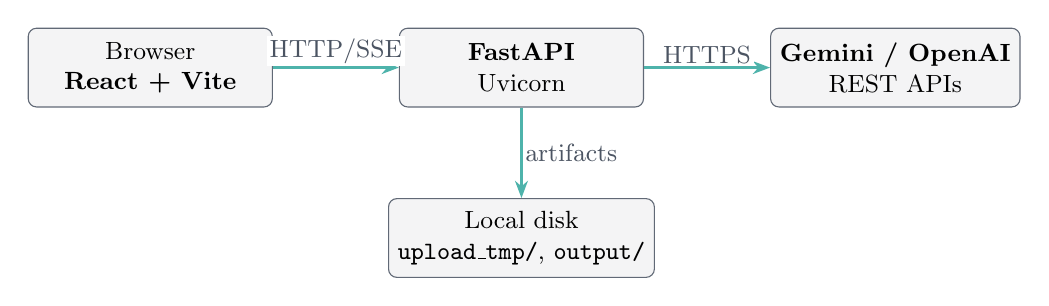
\begin{tikzpicture}[
    font=\small,
    box/.style={draw=BrandSlate!70,rounded corners=3pt,fill=BrandSlate!5,minimum width=3.1cm,minimum height=1cm,align=center},
    arr/.style={-{Stealth[length=2.2mm]},thick,BrandTeal!80},
    lbl/.style={midway,fill=white,inner sep=1pt,text=BrandSlate!80},
  ]
    \node[box] (ui) {Browser\\\textbf{React + Vite}};
    \node[box,right=1.6cm of ui] (api) {\textbf{FastAPI}\\Uvicorn};
    \node[box,right=1.6cm of api] (llm) {\textbf{Gemini / OpenAI}\\REST APIs};
    \node[box,below=1.15cm of api] (disk) {Local disk\\\texttt{upload\_tmp/}, \texttt{output/}};
    \draw[arr] (ui) -- node[lbl,above] {HTTP/SSE} (api);
    \draw[arr] (api) -- node[lbl,above] {HTTPS} (llm);
    \draw[arr] (api) -- node[lbl,right] {artifacts} (disk);
  \end{tikzpicture}
  \caption{Logical components: the API is the single integration point for models and disk.}
\end{figure}

\subsection{Technology stack}
\begin{tabularx}{\linewidth}{@{}lX@{}}
  \toprule
  \textbf{Layer} & \textbf{Choice} \\
  \midrule
  Frontend & React~19, Vite, TypeScript, Tailwind CSS~v4, Lucide icons \\
  Backend & Python~3.11+, FastAPI, Uvicorn, \texttt{asyncio} background tasks \\
  Media AI & \texttt{google-genai} (file upload + generate), optional OpenAI transcription \\
  Deck build & \texttt{python-pptx} \\
  \bottomrule
\end{tabularx}

% =============================================================================
\section{End-to-end data flow}
% =============================================================================

\begin{enumerate}[leftmargin=*]
  \item \textbf{POST} \texttt{/api/process} with \texttt{multipart/form-data}: optional \texttt{file}, booleans \texttt{use\_sample\_file}, \texttt{force\_demo\_summary}.
  \item Handler \textbf{registers} a UUID job, \textbf{streams} the file to \texttt{backend/upload\_tmp/\{job\_id\}\{ext\}}, returns \texttt{200} with \texttt{job\_id} and header \texttt{X-API-Revision}.
  \item \texttt{asyncio.create\_task} runs \texttt{run\_pipeline}:
  \begin{itemize}
    \item \textbf{Text upload:} read UTF-8 from the temp path.
    \item \textbf{Media:} \texttt{transcribe\_media} uploads to Gemini (resumable protocol) or OpenAI, waits until file state is active, then requests a plain-text transcript.
    \item \texttt{extract\_transcript\_text} normalizes content; \texttt{transcript.txt} is written under \texttt{backend/output/\{job\_id\}/}; SSE \texttt{artifact\_written}.
    \item \textbf{Summarise} with LLM or demo template; result coerced to schema.
    \item \textbf{Build} \texttt{meeting\_briefing.pptx} and \texttt{summary.json} (JSON may include \texttt{\_briefing\_meta}).
    \item SSE \texttt{completed} carries relative download paths.
  \end{itemize}
  \item Temp upload file is \textbf{deleted} in a \texttt{finally} block.
  \item Client subscribes to \texttt{GET /api/jobs/\{id\}/stream} and renders events until terminal state.
\end{enumerate}

% =============================================================================
\section{Backend modules (detailed)}
% =============================================================================

\subsection{\texttt{app/main.py}}
\begin{itemize}
  \item CORS for localhost Vite ports; optional \texttt{CORS\_EXTRA\_ORIGINS}.
  \item \texttt{GET /} and \texttt{GET /api} discovery JSON to avoid bare 404s.
  \item \texttt{/api/health}: key presence flags, \texttt{gemini\_http} timeout diagnostics, effective \texttt{gemini\_model}, \texttt{app\_main\_file} path for ``wrong clone'' debugging.
  \item \texttt{/api/process}: chunked upload; \texttt{kickoff} safety net logs unexpected exceptions.
  \item SSE generator: initial \textbf{snapshot} includes \texttt{error} or completed download URLs for late subscribers; heartbeats every 120\,s idle window.
\end{itemize}

\subsection{\texttt{app/pipeline.py}}
In-memory \texttt{jobs} registry; \texttt{broadcast} fan-out to subscriber queues; \texttt{run\_pipeline} orchestration. \textbf{Upload always wins} over bundled sample when both could apply.

\subsection{\texttt{app/summarizer.py}}
\begin{itemize}
  \item \textbf{Gemini:} \texttt{Client(api\_key=..., vertexai=False, http\_options=...)} plus shared \texttt{httpx.Client} for long uploads.
  \item \texttt{summary\_input\_char\_limit()} from \texttt{GEMINI\_SUMMARY\_INPUT\_CHARS} (default large window).
  \item \texttt{\_coerce\_summary\_response}: schema enforcement without injecting demo BrightLane text.
  \item Transcription prompt asks for plain dialogue; summary prompt demands transcript grounding.
\end{itemize}

\subsection{\texttt{app/slides\_builder.py}}
Maps JSON fields to a \textbf{styled} deck: dark slate background, teal accents, titled sections for executive summary, objectives, actions, next steps, and human review---visually aligned with the web UI.

\subsection{\texttt{app/transcript\_clean.py}}
Removes email scaffolding when a synthetic marker or timestamp pattern is detected.

\subsection{\texttt{app/env\_load.py}}
Loads \texttt{.env} with \texttt{utf-8-sig} for Windows BOM tolerance.

\subsection{\texttt{app/\_version.py}}
Monotonic \texttt{API\_REVISION} string for deployment verification.

% =============================================================================
\section{JSON schema and metadata}
% =============================================================================

\subsection{Primary fields}
\begin{lstlisting}[language=json]
{
  "executive_summary": "string",
  "objectives": ["...", "...", "..."],
  "actionable_items": ["...", "...", "..."],
  "next_steps": ["...", "...", "..."],
  "human_review_notes": "string"
}
\end{lstlisting}

\subsection{\texttt{\_briefing\_meta}}
Written alongside the model output for audit:
\begin{itemize}
  \item \texttt{transcript\_character\_count}
  \item \texttt{summarized\_character\_cap}, \texttt{summarized\_chars\_effective}
  \item \texttt{transcript\_truncated\_for\_summary}
  \item \texttt{source} filename or sample label
\end{itemize}

% =============================================================================
\section{HTTP API reference}
% =============================================================================

\begin{longtable}{@{}llp{7.2cm}@{}}
  \toprule
  \textbf{Method} & \textbf{Path} & \textbf{Description} \\
  \midrule
  \endhead
  GET & \texttt{/} & Service index with endpoint list. \\
  GET & \texttt{/api} & Same, under \texttt{/api} prefix (proxy-friendly). \\
  GET & \texttt{/docs} & FastAPI Swagger UI. \\
  GET & \texttt{/api/health} & Liveness, keys, Gemini timeouts, model id, revision. \\
  POST & \texttt{/api/process} & Multipart job start; returns \texttt{job\_id}. \\
  GET & \texttt{/api/jobs/\{id\}/stream} & SSE (\texttt{text/event-stream}). \\
  GET & \texttt{/api/jobs/\{id\}/download/transcript} & \texttt{transcript.txt} \\
  GET & \texttt{/api/jobs/\{id\}/download/pptx} & \texttt{meeting\_briefing.pptx} \\
  GET & \texttt{/api/jobs/\{id\}/download/json} & \texttt{summary.json} \\
  \bottomrule
\end{longtable}

\subsection{SSE event names}
\texttt{job\_started}, \texttt{ingest}, \texttt{transcribing}, \texttt{transcript\_ready}, \texttt{artifact\_written}, \texttt{summarizing}, \texttt{building\_slides}, \texttt{completed}, \texttt{error}, \texttt{subscribed}, \texttt{heartbeat}.

% =============================================================================
\section{Environment variables}
% =============================================================================

\subsection{Backend (\texttt{backend/.env})}
\begin{tabularx}{\linewidth}{@{}lX@{}}
  \toprule
  \textbf{Variable} & \textbf{Role} \\
  \midrule
  \texttt{GEMINI\_API\_KEY} / \texttt{GOOGLE\_API\_KEY} & AI Studio key \\
  \texttt{GEMINI\_MODEL} & Model id (default \texttt{gemini-2.5-flash}; 2.0 Flash retired for new users) \\
  \texttt{GEMINI\_HTTP\_TIMEOUT\_SEC} & Client HTTP deadline (seconds; converted to ms for SDK) \\
  \texttt{GEMINI\_FILE\_ACTIVE\_DEADLINE\_SEC} & Poll until uploaded file is active \\
  \texttt{GEMINI\_SUMMARY\_INPUT\_CHARS} & Max transcript chars sent to summariser \\
  \texttt{OPENAI\_API\_KEY} & Optional; summary + Whisper path \\
  \texttt{CORS\_EXTRA\_ORIGINS} & Extra allowed browser origins \\
  \bottomrule
\end{tabularx}

\subsection{Frontend (Vite)}
\begin{tabularx}{\linewidth}{@{}lX@{}}
  \toprule
  \textbf{Variable} & \textbf{Role} \\
  \midrule
  \texttt{VITE\_PROXY\_API} & Target for dev proxy (\texttt{http://127.0.0.1:8787} on Windows backend) \\
  \texttt{VITE\_API\_URL} & Optional direct API base; empty = same-origin \texttt{/api} \\
  \texttt{VITE\_UPLOAD\_TIMEOUT\_MS} & Client-side upload abort (default 30\,min) \\
  \texttt{VITE\_USE\_WSL\_API} & Resolve WSL LAN IP when needed \\
  \bottomrule
\end{tabularx}

% =============================================================================
\section{Networking and local development}
% =============================================================================

\begin{itemize}
  \item \textbf{WSL2:} bind Uvicorn to \texttt{0.0.0.0} when accessed from Windows; prefer \texttt{127.0.0.1} port forwarding when it works to avoid Chrome Private Network Access friction.
  \item \textbf{Vite proxy:} extended \texttt{timeout} / \texttt{proxyTimeout} for long SSE and uploads.
  \item \textbf{API keys:} never commit \texttt{.env}; rotate keys exposed in logs or chat (Google may return HTTP~403 for leaked keys).
\end{itemize}

% =============================================================================
\section{Security and privacy (POC level)}
% =============================================================================

\begin{itemize}
  \item Transcripts and media are ephemeral on disk under developer control; outputs live in \texttt{backend/output/}.
  \item Production would add tenant isolation, encryption at rest, retention, audit logs, and managed secrets.
\end{itemize}

% =============================================================================
\section{Operational scripts}
% =============================================================================

\begin{itemize}
  \item \texttt{backend/run\_dev\_wsl.sh} --- sync venv, install requirements, Uvicorn on \texttt{0.0.0.0:8787}.
  \item \texttt{run\_backend\_wsl.sh} (repo root) --- convenience wrapper.
  \item Windows: \texttt{.venv\textbackslash Scripts\textbackslash python -m uvicorn app.main:app --reload --host 127.0.0.1 --port 8787} from \texttt{backend/}.
\end{itemize}

% =============================================================================
\section{Repository layout (essential)}
% =============================================================================

\begin{lstlisting}
backend/app/              # Application package
backend/output/         # Per-job artifacts (gitignored)
backend/upload_tmp/     # Ephemeral uploads (gitignored)
frontend/src/           # React source
deliverables/           # Stakeholder Markdown docs
Syntethic_AI_Transcript.txt   # Bundled sample transcript
docs/latex/             # This document
\end{lstlisting}

% =============================================================================
\section{Synthetic sample scenario}
% =============================================================================

\texttt{Syntethic\_AI\_Transcript.txt} supplies the ``BrightLane Retail'' narrative for demos \textbf{without} media. The \textbf{deterministic fallback} summary matches that file when \texttt{force\_demo\_summary} is enabled or no LLM keys exist; it is \textbf{not} mixed into real LLM output after coercion fixes.

% =============================================================================
\section{Future work}
% =============================================================================

\begin{itemize}
  \item Cloud Run (or similar) for API + bounded workers; signed URLs for downloads.
  \item Optional second-pass validation: LLM self-check against transcript quotes.
  \item User-selectable slide themes and languages.
\end{itemize}

% =============================================================================
\section{Building this PDF}
% =============================================================================

From \texttt{docs/latex}:
\begin{lstlisting}[language=bash]
pdflatex -interaction=nonstopmode meeting-slides-poc.tex
pdflatex -interaction=nonstopmode meeting-slides-poc.tex
\end{lstlisting}
Or \texttt{latexmk -pdf meeting-slides-poc.tex}. See \texttt{README.txt} in the same folder.

\end{document}
